\documentclass[conference,a4paper]{IEEEtran}
\IEEEoverridecommandlockouts
\usepackage{cite}
\usepackage{amsmath,amssymb}
\usepackage{graphicx}
\usepackage{booktabs}
\usepackage{xcolor}
\usepackage{tikz}
\usetikzlibrary{positioning,arrows.meta,fit,calc}
\graphicspath{{../paper/}{./}}
\newcommand{\pending}[1]{\textcolor{red}{[#1]}}
\newcommand{\RecallMsixOOF}{0.47 [0.25, 0.66]}
\newcommand{\RecallGBMOOF}{0.25 [0.20, 0.30]}
\newcommand{\DiffOOF}{+0.22 [+0.04, +0.38]}
\newcommand{\PalignMedian}{1.8\%}
\newcommand{\NexpCHIME}{$5.3\times10^{-6}$}
\newcommand{\NexpCHIMEbias}{$1.2\times10^{-4}$}
\newcommand{\GainAllSky}{$\sim$50}
\newcommand{\GainTenYr}{1.4--1.8}
\newcommand{\HostSens}{$-$19\%}
\newcommand{\HostSensTau}{$-$13\%}
\newcommand{\NexpEcho}{$3.2\times10^{-5}$}
\newcommand{\NexpEchoPair}{$1.5\times10^{-5}$}
\newcommand{\FarHeldOut}{1 of 166{,}000 held-out scrambles}
\newcommand{\FarRateUp}{$2.9\times10^{-5}$}
\newcommand{\FarSearchUp}{0.002}
\newcommand{\ReproHashes}{7/7 match}
\newcommand{\ReproMsix}{0.668}
\newcommand{\SthreeFPRMsix}{1.4\% [0.1, 4.0]}
\newcommand{\SthreeFPRGBM}{1.3\% [0.2, 2.8]}
\newcommand{\SthreeTwinMsix}{0.76 against 0.87}
\newcommand{\SthreeTwinGBM}{0.83 against 0.83}
\newcommand{\EhSim}{1.94}
\newcommand{\EhReal}{1.10 [0.20, 2.55]}
\newcommand{\SthreeFPRMsixSeeds}{1.4, 1.9, 1.6\%}
\newcommand{\SthreeFPRMsixHi}{5\%}
\newcommand{\GapMsix}{+0.6 to +1.2 points}
\newcommand{\GapBaseMax}{0.5 points}
\newcommand{\BoneLowReal}{6.2, 3.8, 2.4\%}
\newcommand{\BoneLowTwin}{5.6, 4.0, 2.5\%}
\newcommand{\SnrLowReal}{16.9}
\newcommand{\SnrLowSim}{13.5}
\newcommand{\EhSimSeeds}{1.9, 1.7, 7.3}
\newcommand{\EhRealSeeds}{1.10, 1.86, 1.53}
\newcommand{\ReproSeeds}{0.668 / 0.649 / 0.616}
\newcommand{\AblSeeds}{3}
\newcommand{\AblFull}{0.644}
\newcommand{\AblNoalign}{0.557, difference $-$0.087 [$-$0.186, $-$0.025]}
\newcommand{\AblHardneg}{0.698, difference +0.053 [$-$0.011, +0.082]}
\newcommand{\AblNoimp}{0.474, difference $-$0.170 [$-$0.254, $-$0.052]}
\newcommand{\ForecastRows}{CHIME, Catalog 2 & $2.9\times10^{-3}$ & $5.3\times10^{-6}$ & $3.2\times10^{-5}$ \\
All-sky, same sources & $2.9\times10^{-3}$ & $2.6\times10^{-4}$ & $6.3\times10^{-4}$ \\
CHIME, Catalog 2, $\gamma=1.5$ & $1.8\times10^{-2}$ & $1.2\times10^{-4}$ & $4.9\times10^{-4}$ \\
All-sky, same sources, $\gamma=1.5$ & $1.8\times10^{-2}$ & $6.1\times10^{-3}$ & $9.3\times10^{-3}$ \\
CHIME-like, 10 yr & $2.8\times10^{-3}$ & $7.4\times10^{-6}$ & $4.9\times10^{-5}$ \\
All-sky, 10 yr & $2.8\times10^{-3}$ & $3.7\times10^{-4}$ & $6.8\times10^{-4}$ \\
CHIME-like, 10 yr, $\gamma=1.5$ & $1.8\times10^{-2}$ & $2.2\times10^{-4}$ & $6.3\times10^{-4}$ \\
All-sky, 10 yr, $\gamma=1.5$ & $1.8\times10^{-2}$ & $7.4\times10^{-3}$ & $9.6\times10^{-3}$ \\}

\newcommand{\SthreeNpairs}{3851}
\newcommand{\SthreeTeamMsix}{0.8--1.4\%}
\newcommand{\AblNoalignR}{0.557}
\newcommand{\AblNoalignD}{$-$0.087 [$-$0.186, $-$0.025]}
\newcommand{\AblNoimpR}{0.474}
\newcommand{\AblNoimpD}{$-$0.170 [$-$0.254, $-$0.052]}
\newcommand{\AblHardnegR}{0.698}
\newcommand{\AblHardnegD}{+0.053 [$-$0.011, +0.082]}
\newcommand{\SthreeRepro}{Repeating this check on the second machine with its own model~6 seeds gives 1.5, 1.3, 1.0\% (3851 pairs), all within the limit, with rank correlations 0.91--0.92 against ceilings 0.87--0.89.}
\newcommand{\RealBurstRepro}{On the second machine, its own model~6 seeds give a real/template ratio of 0.97 [0.91, 1.08].}
\newcommand{\ForecastCompact}{Catalog 2, as observed & $5\times10^{-6}$ & $3\times10^{-5}$ & $3\times10^{-4}$ \\
Catalog 2, $\gamma=1.5$ & $1\times10^{-4}$ & $5\times10^{-4}$ & $6\times10^{-3}$ \\
10-yr survey & $7\times10^{-6}$ & $5\times10^{-5}$ & $4\times10^{-4}$ \\
10-yr survey, $\gamma=1.5$ & $2\times10^{-4}$ & $6\times10^{-4}$ & $7\times10^{-3}$ \\}
\newcommand{\NexpLo}{$5\times10^{-6}$}
\newcommand{\NexpHi}{$1\times10^{-4}$}
\newcommand{\GainAllSkyOne}{50}


\begin{document}

\title{Siamese Correlation Networks for Identifying Gravitationally Lensed Fast Radio Bursts: Real-Data Validation and the Limits Set by Survey Geometry}

\author{\IEEEauthorblockN{Author names withheld for review}
\IEEEauthorblockA{Affiliations to be added}}

\maketitle

\begin{abstract}
A fast radio burst (FRB) lensed by a foreground galaxy would reach Earth twice, days to months apart, with the two copies
differing only by propagation effects. Recognising such copies among the thousands of bursts from repeating sources is a
pairwise verification problem with no real positive examples. We build a semi-synthetic benchmark from all 981 public
dynamic spectra of the 83 repeating sources in the CHIME/FRB Catalog~2, with real noise, measured signal-to-noise ratios and
\emph{impostor} pairs of different bursts that share a propagation imprint. A 259k-parameter Siamese encoder that aligns two
feature maps with a differentiable correlation layer before fusing them recovers \RecallMsixOOF\ of lensed pairs at 1\%
false-positive rate in source-grouped cross-validation, against \RecallGBMOOF\ for the best physics- or feature-based
baseline. Ablations over three seeds show that both the alignment layer and impostor training are needed. Because no real
lensed pair exists, we validate on real data in three ways: real cross-source pairs serve as true negatives, scored against
per-pair simulated twins; two copies of a real burst stand in for lensed pairs; and the whole pipeline is reproduced on a
second machine. Finally, we show that survey geometry, not the classifier, limits discovery: a transit telescope records the
copies of a repeater's bursts only for the \PalignMedian\ of lenses whose delay is close to a whole number of sidereal days,
so an all-sky monitor would find about \GainAllSky$\times$ more lensed repeaters than CHIME from the same sources.
\end{abstract}

\begin{IEEEkeywords}
Siamese networks, pairwise verification, simulation-to-real transfer, signal processing, radio astronomy, gravitational lensing
\end{IEEEkeywords}

\section{Introduction}
Fast radio bursts are millisecond radio flashes from distant galaxies; some sources repeat thousands of times. If a galaxy
lies close to the line of sight, gravitational lensing produces two images of the source, and every burst then arrives twice,
separated by a fixed delay of days to months~\cite{Li2018,Wucknitz2021}. A confirmed lensed FRB would measure the Hubble
constant and test dark-matter models, but none is known~\cite{Chang2024,Kader2022,Leung2022,Krochek2022}.

Finding one is a pairwise verification problem: given two bursts from the same sky position, are they two copies of one
burst, or two different bursts from the same repeating source? This is hard for three reasons. There are no real positive
examples, so any classifier is trained on simulation and must be validated on real data without labels. The negatives are
adversarial: different bursts of one source can share a spectral envelope imposed by plasma lensing, or a scintillation
pattern, and look like copies. And the decision must hold at very low false-positive rates, because the prior probability of
lensing is about $10^{-3}$ per source.

Lensed-pair classifiers exist for gravitational waves~\cite{Goyal2021,Zhang2026}, where Siamese networks fuse paired
features by their absolute difference and product. FRB lensing searches have so far used auto- and cross-correlation
statistics~\cite{Kader2022,Chang2024}. Our contributions are:
\begin{enumerate}
\item a semi-synthetic pair benchmark built from all public CHIME/FRB Catalog~2 repeater spectra, with impostor negatives and
frozen, hash-checked evaluation sets (Section~\ref{sec:data});
\item a Siamese correlation network that aligns feature maps before fusing them, with an ablation study (Sections~\ref{sec:method}, \ref{sec:results});
\item a validation protocol for a detector without real positives: true-negative transfer with per-pair twins, a real-burst
positive proxy, and an independent reproduction (Section~\ref{sec:validation});
\item an analysis of where such a detector can work, which shows that transit telescopes rarely record both copies and that
sky coverage, not classifier accuracy, limits discovery (Section~\ref{sec:geometry}).
\end{enumerate}

\section{Related Work}
\textbf{Siamese verification.} Siamese networks decide whether two inputs share an identity by comparing embeddings from one
shared encoder, from signature verification~\cite{Bromley1993} to one-shot recognition~\cite{Koch2015}. Most compare global
vectors, which discards the relative position of features; our classic Siamese baseline (5) is of this kind. Correlation
layers that compare feature maps over a range of displacements were introduced for optical flow~\cite{Dosovitskiy2015}; we
use one to estimate and remove the residual time shift between two bursts before comparison.

\textbf{Lensed-pair identification.} For gravitational waves, lensed event pairs have been identified with a DenseNet and
gradient boosting~\cite{Goyal2021} and with a Siamese residual network that fuses features by absolute difference and
product~\cite{Zhang2026}; the latter notes the need for adaptation to real detector data. For FRBs, lensing searches have
used auto- and cross-correlation statistics~\cite{Kader2022,Chang2024,Krochek2022}, and machine learning has been used to
classify repeating from non-repeating sources~\cite{Chen2022}, not to identify lensed copies.

\textbf{Simulation-to-real transfer.} Detectors trained on simulation are commonly made robust by randomising nuisances
during training~\cite{Tobin2017}. Without real positives, transfer must also be checked on real data; we do so with real
negatives, per-pair twins and a real-signal positive proxy.

\section{Data and Benchmark}
\label{sec:data}
\textbf{Real inputs.} We use the Stokes-I dynamic spectra of all 981 bursts of the 83 repeating sources in CHIME/FRB
Catalog~2~\cite{CHIME2025cat2}, at 0.983\,ms and 400--800\,MHz. Each burst is binned to 256 frequency channels $\times$ 160
time samples around the emission and normalised by its off-pulse noise. The catalogue's fitted burst models serve as
noise-free templates (950 eligible), and off-pulse columns of each file, mirror-tiled, serve as real backgrounds (856).

\textbf{Pair classes.} A \emph{lensed} pair places one template twice; a \emph{repeat} pair places two templates of one
source; an \emph{unrelated} pair takes templates of two sources; an \emph{impostor} pair is a repeat pair that shares a
propagation imprint: member B inherits member A's 25-MHz-smoothed spectral envelope (I1, mimicking a plasma lens), both share
one scintillation pattern (I2), or both. Each member is injected at a measured matched-filter S/N on a different real
background, with its own time shift ($\pm10$ samples), residual dispersion, scattering and scintillation, so that only
burst identity separates lensed from repeat pairs. Single-member statistics cannot tell the classes apart (probe AUC
$\le0.53$).

\begin{figure*}[t]
\centering
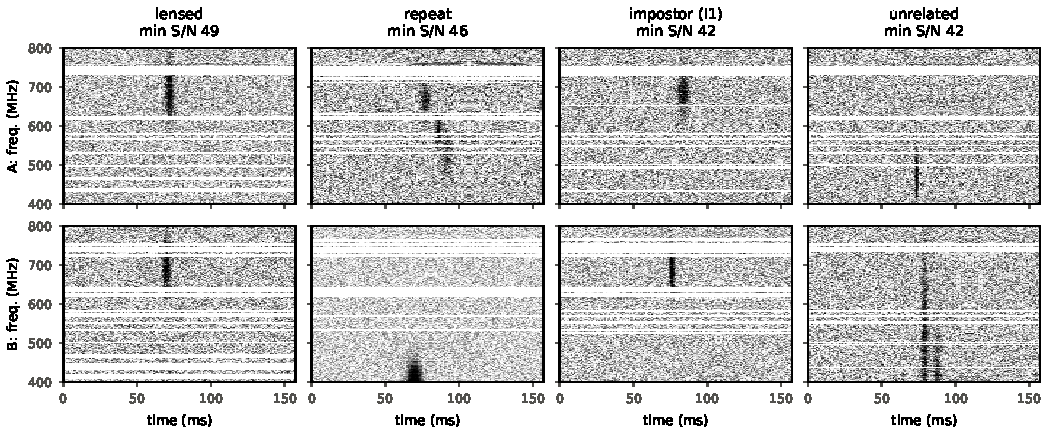
\includegraphics[width=\textwidth]{fig_examples.pdf}
\caption{One validation pair of each class at similar S/N (rows: members A and B; white rows: masked radio-frequency
interference). A lensed pair repeats one burst on different real backgrounds with independent nuisances; a repeat pair shows
two bursts of one source; an impostor pair shows two bursts of one source where B inherits A's spectral envelope, mimicking a
plasma lens; an unrelated pair comes from two sources. The detector must separate the first column from the other three at a
1\% false-positive rate.}
\label{fig:examples}
\end{figure*}

\textbf{Splits and frozen sets.} Sources are split 60/20/20 into train, validation and test. Validation and test sets of 4000
pairs, and ``bright'' sets with pair minimum S/N\,$\ge25$ (the pre-registered headline bin), are regenerated from fixed seeds
and checked against stored SHA-256 hashes. The test split stays sealed under a pre-registered blind protocol; all numbers
below are development results on sources never used for training.

\textbf{Metric.} Recall of lensed pairs at 1\% false-positive rate against repeat and impostor pairs, with 95\% intervals
from a source-level bootstrap that recomputes the threshold in every resample.

\section{Method}
\label{sec:method}
\begin{figure*}[t]
\centering
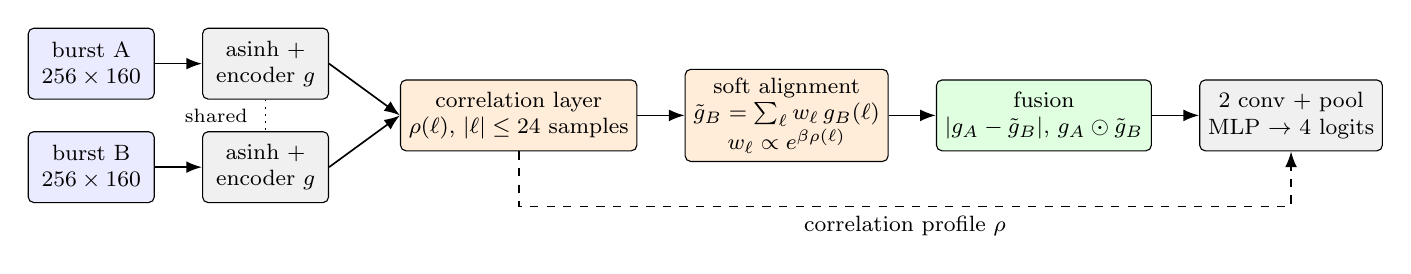
\begin{tikzpicture}[font=\footnotesize, node distance=4mm and 6mm,
  box/.style={draw, rounded corners=2pt, align=center, minimum height=9mm, minimum width=16mm, inner sep=3pt, fill=#1},
  box/.default=white, ar/.style={-{Latex[length=2mm]}, semithick}]
\node[box=blue!8] (a) {burst A\\$256\times160$};
\node[box=blue!8, below=of a] (b) {burst B\\$256\times160$};
\node[box=gray!12, right=of a] (ea) {asinh +\\encoder $g$};
\node[box=gray!12, right=of b] (eb) {asinh +\\encoder $g$};
\coordinate (mid) at ($(ea.east)!0.5!(eb.east)$);
\node[box=orange!15, right=9mm of mid] (corr) {correlation layer\\$\rho(\ell)$, $|\ell|\le24$ samples};
\node[box=orange!15, right=of corr] (al) {soft alignment\\$\tilde g_B=\sum_\ell w_\ell\, g_B(\ell)$\\$w_\ell\propto e^{\beta\rho(\ell)}$};
\node[box=green!12, right=of al] (fu) {fusion\\$|g_A-\tilde g_B|$,\ $g_A\odot\tilde g_B$};
\node[box=gray!12, right=of fu] (hd) {2 conv + pool\\MLP $\to$ 4 logits};
\draw[ar] (a) -- (ea); \draw[ar] (b) -- (eb);
\draw[ar] (ea.east) -- (corr.west); \draw[ar] (eb.east) -- (corr.west);
\draw[ar] (corr) -- (al); \draw[ar] (al) -- (fu); \draw[ar] (fu) -- (hd);
\draw[ar, dashed] (corr.south) -- ++(0,-7mm) -| node[pos=0.25, below]{correlation profile $\rho$} (hd.south);
\draw[dotted, semithick] (ea.south) -- node[left, font=\scriptsize, xshift=-1mm]{shared} (eb.north);
\end{tikzpicture}
\caption{Model 6, the Siamese correlation network. A weight-shared encoder maps each burst to a $64\times16\times80$
feature map at two-sample time resolution; a correlation layer over $\pm24$ samples measures the residual delay and softly
aligns B to A with a learned temperature $\beta$; the aligned maps are fused by absolute difference and product. The
correlation profile also feeds the head. Both directions are computed and averaged, so the score is symmetric in A and B.}
\label{fig:arch}
\end{figure*}

\textbf{Benchmark ladder.} All methods score the same pairs, averaged over both member orders:
(1)~normalised cross-correlation in the on-pulse box, maximised over $\pm24$ lags, with 1, 4 or 16 channel blocks;
(2)~a physics statistic that fits one member to the other over scattering time, residual dispersion, lag and amplitude;
(3)~gradient-boosted trees (GBM) on seven measured burst properties per member (best of 1--3, the comparator);
(4)~a two-channel CNN; (5)~a classic Siamese network comparing vector embeddings;
(6)~our Siamese correlation network (Fig.~\ref{fig:arch}); and (7)~cross-attention between time--frequency patches.

\textbf{Model 6.} Inputs pass through $\mathrm{asinh}$ to compress the dynamic range. The encoder $g$ has four
$5\times3$ convolution blocks with group normalisation, reducing $256\times160$ to $64$ channels $\times\,16\times80$ while
keeping two-sample time resolution, because lensed copies differ by residual time shifts. The correlation layer computes the
normalised correlation $\rho(\ell)$ of the two maps over lags $|\ell|\le12$ encoder steps ($\pm24$ samples), forms softmax
weights $w_\ell\propto\exp(\beta\rho(\ell))$ with learned $\beta$, and aligns $g_B$ as $\sum_\ell w_\ell\,g_B(\ell)$.
Fusion concatenates $|g_A-g_B|$ and $g_A\odot g_B$, two convolution blocks and mean/max pooling follow, and an MLP receives the
pooled features with $\rho$. The model has 259k parameters.

\textbf{Training.} All learned models are trained for 20\,000 steps of 64 pairs generated on the fly from training sources
(half with S/N floor 10, half 25), with four-class cross-entropy, AdamW (learning rate $10^{-3}$, weight decay $10^{-4}$),
1000 warm-up steps and cosine decay; the checkpoint is selected on the validation bright set. The lensed score is the
log-odds of the lensed class against the other three.

\section{Validation Without Real Positives}
\label{sec:validation}
\textbf{Grouped folds.} Because the validation interval was wide, a pre-registered rule moved the primary comparison to five
source-grouped folds: each source is scored by a model that never saw it.

\textbf{True-negative transfer.} Two bursts from different sources cannot be lensed copies, so real cross-source pairs are
labelled negatives that can be scored without breaking the blind protocol. For each such pair we simulate five
\emph{twins} from the same two templates at their measured S/N, and set the threshold at the twins' 99th percentile; the
pre-registered criterion is a real false-positive rate of at most 2\%. Twin matching matters: with a threshold from
generic simulated pairs, cross-correlation appears to fail below S/N\,25 (real rate \BoneLowReal\ for its three variants),
yet its twins fail just as often (\BoneLowTwin) because the real pairs there are brighter than generic ones (median S/N
\SnrLowReal\ vs \SnrLowSim). The ``failure'' is sample composition, not a simulation gap.

\textbf{Real-burst positives.} As a stand-in for lensed pairs, two copies of a real burst's cutout, with its fine structure,
are injected with independent nuisances on different backgrounds, alongside template copies and noise-only copies made with
the same random draws.

\textbf{Reproduction.} A second machine re-downloaded and re-processed all 981 spectra, rebuilt the injection cache and
regenerated the frozen sets, then retrained model 6 and repeated the checks.

\section{Results}
\label{sec:results}
\begin{table}[t]
\caption{Recall at 1\% FPR, lensed vs repeat + impostor, S/N\,$\ge25$, validation sources (95\% source bootstrap).}
\label{tab:main}
\centering
\setlength{\tabcolsep}{2pt}
\resizebox{\columnwidth}{!}{%
\begin{tabular}{lcc}
\toprule
Method & Fixed split (3 seeds) & Grouped folds (OOF) \\
\midrule
(1) Cross-correlation, 16 blocks & 0.171 [0.115, 0.245] & -- \\
(2) Physics fit, 16 blocks & 0.164 [0.119, 0.235] & -- \\
(3) Feature GBM & 0.285 [0.180, 0.401] & 0.246 [0.199, 0.297] \\
(4) Two-channel CNN & 0.423 / 0.409 / 0.407 & -- \\
(5) Classic Siamese & 0.500 / 0.559 / 0.541 & -- \\
(7) Cross-attention & 0.471 / 0.013$^a$ / 0.579 & -- \\
(6) Ours & \textbf{0.701 / 0.698 / 0.684} & \textbf{0.467 [0.253, 0.662]} \\
\midrule
(6) $-$ (3), paired & +0.394 [+0.226, +0.542] & +0.220 [+0.035, +0.381] \\
(6) reproduction$^b$ & \ReproSeeds & -- \\
\bottomrule
\end{tabular}}\\[2pt]
\parbox{\columnwidth}{\footnotesize $^a$Collapsed to a plateau (one of three seeds). $^b$Second machine, different data-loader
worker count; seed 0 inside the pre-registered range 0.66--0.72, the mean 0.05 below the original seeds.}
\end{table}

\textbf{Benchmark.} Table~\ref{tab:main} shows that every learned model beats the physics and feature baselines, and model 6
leads all of them, by +0.39 recall over the GBM on the fixed split and +0.22 [+0.04, +0.38] in grouped folds. At the 1\%
threshold its false positives are almost all I1 impostors, which share a spectral envelope by construction; plain repeats are
rarely confused. Model 6 classifies 95\% of lensed pairs of unseen sources correctly, while its confusion of repeat and
unrelated pairs on unseen sources (32\% correct vs 86\% on seen) shows that part of its capacity memorises source identity;
training variants that remove this incentive are in progress.

\begin{table}[t]
\caption{Ablations of model 6 (three seeds each): seed-mean recall and paired difference from the full model, validation bright set.}
\label{tab:abl}
\centering
\setlength{\tabcolsep}{3pt}
\begin{tabular}{lcc}
\toprule
Variant & Recall & Difference [95\%] \\
\midrule
Full model & \AblFull & -- \\
No alignment (correlation off) & \AblNoalignR & \AblNoalignD \\
No impostors in training & \AblNoimpR & \AblNoimpD \\
Hard-negative repeats & \AblHardnegR & \AblHardnegD \\
\bottomrule
\end{tabular}
\end{table}

\begin{figure}[t]
\centering
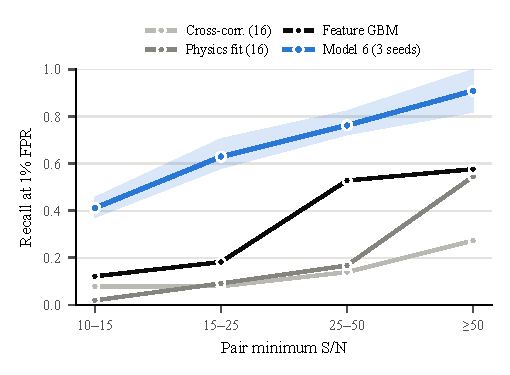
\includegraphics[width=\columnwidth]{fig_snr.pdf}
\caption{Recall at 1\% FPR by pair minimum S/N on the frozen validation set (529, 330, 108 and 33 lensed pairs per bin).
Model 6: mean and range of three seeds trained on the second machine, with checkpoints selected on the separate bright
set. Its largest relative gain is at low S/N, the bin with the most pairs.}
\label{fig:snr}
\end{figure}

The gain holds at every S/N (Fig.~\ref{fig:snr}) and is largest in relative terms at the faint end, where model 6
recovers about 0.41 of lensed pairs against 0.12 for the GBM.

\textbf{Ablations.} Removing the alignment, or training without impostors, lowers recall in every seed
(Table~\ref{tab:abl}). Without impostors the network mistakes envelope-sharing bursts of one source for copies. Oversampling
template-similar repeats helps slightly in every seed, but the interval includes zero, and on a closed-form benchmark this
scheme biased a learned likelihood ratio low by about 1\,dex, so we do not adopt it without a correction.

\textbf{Transfer to real negatives.} On the \SthreeNpairs\ real cross-source pairs of the validation sources, all 15
trained models and baselines meet the twin-threshold criterion in both S/N bins once short real windows are filled with
off-pulse noise like the simulated backgrounds: model 6 reaches \SthreeTeamMsix\ in the headline bin (GBM 0.009), and its real-to-twin rank
correlation reaches the twin-to-twin ceiling. Before the fill, model 6 flagged pairs whose windows shared the same blank
edges, a format mismatch that a twin test exposed and the fill removed. \SthreeRepro

\textbf{Real-burst positives.} At injected S/N\,25, model 6 recovers 0.663 of real-burst copies against 0.691 of template
copies (ratio 0.96 [0.89, 1.06]) and none of the noise-only copies, while the GBM recovers 0.178. The classic Siamese network
drops to a ratio of 0.72--0.84, so it relies on template smoothness and model 6 does not. \RealBurstRepro

\section{Where Can Such a Detector Work?}
\label{sec:geometry}
A lensed repeater can also be found without a classifier: a galaxy lens fixes the delay to far better than the 4\,ms
catalogue timing, so two burst pairs that share one delay are already significant. We calibrated this timing test on burst
lists scrambled by whole sidereal days and confirmed its false-alarm rate on independent scrambles (\FarHeldOut).

\begin{figure}[t]
\centering
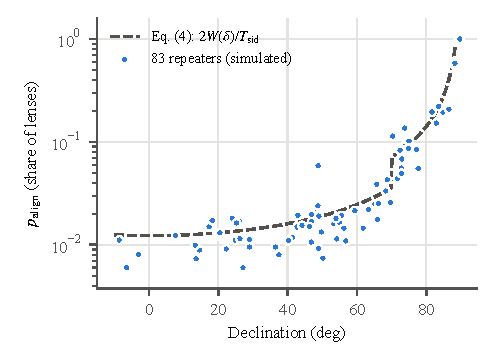
\includegraphics[width=0.92\columnwidth]{fig_transit.pdf}
\caption{Share of galaxy-lens delays for which CHIME records the copies of a repeater's bursts, for the 83 Catalog~2
repeaters (points, simulated with each source's own burst times, exposure and redshift) and the analytic window width
(dashed).}
\label{fig:transit}
\end{figure}

Both the classifier and the timing test need the copies to be recorded. CHIME is a transit telescope: it sees a source for
minutes per day, and every recorded burst arrives within minutes of transit. The copy of each burst then arrives at the same
hour-angle offset, $24\,\mathrm{h}\times\mathrm{frac}(\Delta t/T_{\rm sid})$, so copies are recorded for all bursts or none,
and only if the delay is within minutes of a whole number of sidereal days. Simulating singular-isothermal-sphere lenses
with each source's redshift, burst times and exposure, this happens for \PalignMedian\ of lenses at the median, following
the analytic window width (Fig.~\ref{fig:transit}). Repeaters therefore do not escape the transit problem known for one-off
bursts~\cite{ConnorRavi2022}. Table~\ref{tab:forecast} gives the expected number of detectable lensed repeaters: the
Catalog~2 sample is expected to hold \NexpCHIME--\NexpCHIMEbias\ (without and with magnification bias), so a null search is
the expected outcome; a 10-year transit survey gains only \GainTenYr$\times$, while an all-sky monitor watching the same
sources gains \GainAllSky$\times$.
\begin{table}[t]
\caption{Expected lensed repeaters among the 83 Catalog~2 sources ($\gamma$: magnification-bias slope).}
\label{tab:forecast}
\centering
\resizebox{\columnwidth}{!}{%
\begin{tabular}{lccc}
\toprule
Survey & $\sum\tau$ & $N_{\rm exp}$ (timing) & $N_{\rm exp}$ ($\ge1$ copy) \\
\midrule
\ForecastRows
\bottomrule
\end{tabular}}
\end{table} The result is robust to the assumed host dispersion
(\HostSens\ in yield). For transit surveys the classifier's role is to vet the rare single recorded copy and to discard
impostors; its full value lies with wide-field arrays such as BURSTT~\cite{Ho2023}.

\section{Discussion and Limitations}
Simulated false-positive rates rank methods, but deployment thresholds must come from real negatives; twin matching is what
makes such a check interpretable, because it separates simulation gaps from differences in sample composition. Our results
are development results: the test split is sealed until the team signs off the propagation model, and the reproduction found
model 6 about 0.05 recall below the original seeds on a second machine, for reasons we have not isolated. The lens model is a
singular isothermal sphere, impostor strength rests on a simulation choice, and the validation set has only 26 sources.

\section{Conclusion}
A small Siamese network that aligns before it compares identifies lensed copies of real FRB spectra far better than physics
and feature baselines, passes real-data checks designed for a detector without real positives, and reproduces on a second
machine. The same analysis shows that transit geometry, not classification accuracy, is the bottleneck for finding lensed
repeaters, which points such detectors to wide-field radio arrays.

\textbf{Reproducibility.} All inputs are public (CHIME/FRB Catalog~2, DOI 10.11570/25.0066). Code, frozen-set manifests and
hashes, pre-registered plans and every result update are in the project repository (link withheld for review).

\pending{Test-split result after team sign-off.}

\bibliographystyle{IEEEtran}
\bibliography{../paper/references}

\end{document}
